% Options for packages loaded elsewhere
% Options for packages loaded elsewhere
\PassOptionsToPackage{unicode}{hyperref}
\PassOptionsToPackage{hyphens}{url}
\PassOptionsToPackage{dvipsnames,svgnames,x11names}{xcolor}
%
\documentclass[
  12pt]{article}
\usepackage{xcolor}
\usepackage[margin=1in]{geometry}
\usepackage{amsmath,amssymb}
\setcounter{secnumdepth}{-\maxdimen} % remove section numbering
\usepackage{iftex}
\ifPDFTeX
  \usepackage[T1]{fontenc}
  \usepackage[utf8]{inputenc}
  \usepackage{textcomp} % provide euro and other symbols
\else % if luatex or xetex
  \usepackage{unicode-math} % this also loads fontspec
  \defaultfontfeatures{Scale=MatchLowercase}
  \defaultfontfeatures[\rmfamily]{Ligatures=TeX,Scale=1}
\fi
\usepackage{lmodern}
\ifPDFTeX\else
  % xetex/luatex font selection
\fi
% Use upquote if available, for straight quotes in verbatim environments
\IfFileExists{upquote.sty}{\usepackage{upquote}}{}
\IfFileExists{microtype.sty}{% use microtype if available
  \usepackage[]{microtype}
  \UseMicrotypeSet[protrusion]{basicmath} % disable protrusion for tt fonts
}{}
\makeatletter
\@ifundefined{KOMAClassName}{% if non-KOMA class
  \IfFileExists{parskip.sty}{%
    \usepackage{parskip}
  }{% else
    \setlength{\parindent}{0pt}
    \setlength{\parskip}{6pt plus 2pt minus 1pt}}
}{% if KOMA class
  \KOMAoptions{parskip=half}}
\makeatother
% Make \paragraph and \subparagraph free-standing
\makeatletter
\ifx\paragraph\undefined\else
  \let\oldparagraph\paragraph
  \renewcommand{\paragraph}{
    \@ifstar
      \xxxParagraphStar
      \xxxParagraphNoStar
  }
  \newcommand{\xxxParagraphStar}[1]{\oldparagraph*{#1}\mbox{}}
  \newcommand{\xxxParagraphNoStar}[1]{\oldparagraph{#1}\mbox{}}
\fi
\ifx\subparagraph\undefined\else
  \let\oldsubparagraph\subparagraph
  \renewcommand{\subparagraph}{
    \@ifstar
      \xxxSubParagraphStar
      \xxxSubParagraphNoStar
  }
  \newcommand{\xxxSubParagraphStar}[1]{\oldsubparagraph*{#1}\mbox{}}
  \newcommand{\xxxSubParagraphNoStar}[1]{\oldsubparagraph{#1}\mbox{}}
\fi
\makeatother

\usepackage{color}
\usepackage{fancyvrb}
\newcommand{\VerbBar}{|}
\newcommand{\VERB}{\Verb[commandchars=\\\{\}]}
\DefineVerbatimEnvironment{Highlighting}{Verbatim}{commandchars=\\\{\}}
% Add ',fontsize=\small' for more characters per line
\usepackage{framed}
\definecolor{shadecolor}{RGB}{241,243,245}
\newenvironment{Shaded}{\begin{snugshade}}{\end{snugshade}}
\newcommand{\AlertTok}[1]{\textcolor[rgb]{0.68,0.00,0.00}{#1}}
\newcommand{\AnnotationTok}[1]{\textcolor[rgb]{0.37,0.37,0.37}{#1}}
\newcommand{\AttributeTok}[1]{\textcolor[rgb]{0.40,0.45,0.13}{#1}}
\newcommand{\BaseNTok}[1]{\textcolor[rgb]{0.68,0.00,0.00}{#1}}
\newcommand{\BuiltInTok}[1]{\textcolor[rgb]{0.00,0.23,0.31}{#1}}
\newcommand{\CharTok}[1]{\textcolor[rgb]{0.13,0.47,0.30}{#1}}
\newcommand{\CommentTok}[1]{\textcolor[rgb]{0.37,0.37,0.37}{#1}}
\newcommand{\CommentVarTok}[1]{\textcolor[rgb]{0.37,0.37,0.37}{\textit{#1}}}
\newcommand{\ConstantTok}[1]{\textcolor[rgb]{0.56,0.35,0.01}{#1}}
\newcommand{\ControlFlowTok}[1]{\textcolor[rgb]{0.00,0.23,0.31}{\textbf{#1}}}
\newcommand{\DataTypeTok}[1]{\textcolor[rgb]{0.68,0.00,0.00}{#1}}
\newcommand{\DecValTok}[1]{\textcolor[rgb]{0.68,0.00,0.00}{#1}}
\newcommand{\DocumentationTok}[1]{\textcolor[rgb]{0.37,0.37,0.37}{\textit{#1}}}
\newcommand{\ErrorTok}[1]{\textcolor[rgb]{0.68,0.00,0.00}{#1}}
\newcommand{\ExtensionTok}[1]{\textcolor[rgb]{0.00,0.23,0.31}{#1}}
\newcommand{\FloatTok}[1]{\textcolor[rgb]{0.68,0.00,0.00}{#1}}
\newcommand{\FunctionTok}[1]{\textcolor[rgb]{0.28,0.35,0.67}{#1}}
\newcommand{\ImportTok}[1]{\textcolor[rgb]{0.00,0.46,0.62}{#1}}
\newcommand{\InformationTok}[1]{\textcolor[rgb]{0.37,0.37,0.37}{#1}}
\newcommand{\KeywordTok}[1]{\textcolor[rgb]{0.00,0.23,0.31}{\textbf{#1}}}
\newcommand{\NormalTok}[1]{\textcolor[rgb]{0.00,0.23,0.31}{#1}}
\newcommand{\OperatorTok}[1]{\textcolor[rgb]{0.37,0.37,0.37}{#1}}
\newcommand{\OtherTok}[1]{\textcolor[rgb]{0.00,0.23,0.31}{#1}}
\newcommand{\PreprocessorTok}[1]{\textcolor[rgb]{0.68,0.00,0.00}{#1}}
\newcommand{\RegionMarkerTok}[1]{\textcolor[rgb]{0.00,0.23,0.31}{#1}}
\newcommand{\SpecialCharTok}[1]{\textcolor[rgb]{0.37,0.37,0.37}{#1}}
\newcommand{\SpecialStringTok}[1]{\textcolor[rgb]{0.13,0.47,0.30}{#1}}
\newcommand{\StringTok}[1]{\textcolor[rgb]{0.13,0.47,0.30}{#1}}
\newcommand{\VariableTok}[1]{\textcolor[rgb]{0.07,0.07,0.07}{#1}}
\newcommand{\VerbatimStringTok}[1]{\textcolor[rgb]{0.13,0.47,0.30}{#1}}
\newcommand{\WarningTok}[1]{\textcolor[rgb]{0.37,0.37,0.37}{\textit{#1}}}

\usepackage{longtable,booktabs,array}
\newcounter{none} % for unnumbered tables
\usepackage{calc} % for calculating minipage widths
% Correct order of tables after \paragraph or \subparagraph
\usepackage{etoolbox}
\makeatletter
\patchcmd\longtable{\par}{\if@noskipsec\mbox{}\fi\par}{}{}
\makeatother
% Allow footnotes in longtable head/foot
\IfFileExists{footnotehyper.sty}{\usepackage{footnotehyper}}{\usepackage{footnote}}
\makesavenoteenv{longtable}
\usepackage{graphicx}
\makeatletter
\newsavebox\pandoc@box
\newcommand*\pandocbounded[1]{% scales image to fit in text height/width
  \sbox\pandoc@box{#1}%
  \Gscale@div\@tempa{\textheight}{\dimexpr\ht\pandoc@box+\dp\pandoc@box\relax}%
  \Gscale@div\@tempb{\linewidth}{\wd\pandoc@box}%
  \ifdim\@tempb\p@<\@tempa\p@\let\@tempa\@tempb\fi% select the smaller of both
  \ifdim\@tempa\p@<\p@\scalebox{\@tempa}{\usebox\pandoc@box}%
  \else\usebox{\pandoc@box}%
  \fi%
}
% Set default figure placement to htbp
\def\fps@figure{htbp}
\makeatother





\setlength{\emergencystretch}{3em} % prevent overfull lines

\providecommand{\tightlist}{%
  \setlength{\itemsep}{0pt}\setlength{\parskip}{0pt}}



 
\usepackage[numbers,sort]{natbib}
\bibliographystyle{unsrtnat}


\usepackage{booktabs,longtable,threeparttable,lineno}
\renewcommand{\baselinestretch}{1.45}
\linenumbers
\makeatletter
\@ifpackageloaded{caption}{}{\usepackage{caption}}
\AtBeginDocument{%
\ifdefined\contentsname
  \renewcommand*\contentsname{Table of contents}
\else
  \newcommand\contentsname{Table of contents}
\fi
\ifdefined\listfigurename
  \renewcommand*\listfigurename{List of Figures}
\else
  \newcommand\listfigurename{List of Figures}
\fi
\ifdefined\listtablename
  \renewcommand*\listtablename{List of Tables}
\else
  \newcommand\listtablename{List of Tables}
\fi
\ifdefined\figurename
  \renewcommand*\figurename{Figure}
\else
  \newcommand\figurename{Figure}
\fi
\ifdefined\tablename
  \renewcommand*\tablename{Table}
\else
  \newcommand\tablename{Table}
\fi
}
\@ifpackageloaded{float}{}{\usepackage{float}}
\floatstyle{ruled}
\@ifundefined{c@chapter}{\newfloat{codelisting}{h}{lop}}{\newfloat{codelisting}{h}{lop}[chapter]}
\floatname{codelisting}{Listing}
\newcommand*\listoflistings{\listof{codelisting}{List of Listings}}
\makeatother
\makeatletter
\makeatother
\makeatletter
\@ifpackageloaded{caption}{}{\usepackage{caption}}
\@ifpackageloaded{subcaption}{}{\usepackage{subcaption}}
\makeatother
\usepackage{bookmark}
\IfFileExists{xurl.sty}{\usepackage{xurl}}{} % add URL line breaks if available
\urlstyle{same}
% fallback for those not using the hyperref driver hyperxmp:
\makeatletter
\@ifundefined{xmpquote}{\newcommand{\xmpquote}[1]{#1}}{}
\makeatother
\hypersetup{
  pdftitle={Recurrent Gap-Time Survival{,} Rank Tests{,} and Competing Risks Analysis: recurSurvTests},
  pdfauthor={John Muschelli},
  colorlinks=true,
  linkcolor={blue},
  filecolor={Maroon},
  citecolor={Blue},
  urlcolor={Blue},
  pdfcreator={LaTeX via pandoc}}


\title{Recurrent Gap-Time Survival, Rank Tests, and Competing Risks
Analysis: \texttt{recurSurvTests}}
\author{John Muschelli}
\date{2026-09-23}
\begin{document}
\maketitle


\subsection{Abstract}\label{abstract}

Nonparametric recurrent-event survival curves are available in the
statistical literature, but openly available implementations of tests
for differences between those curves have been limited.
\texttt{recurSurvTests} provides R implementations for estimating and
comparing recurrent curves on their intended scales: (i) Wang--Chang
marginal recurrent gap-time survival and Luo--Huang weighted-risk-set
rank tests, (ii) the Pena--Strawderman--Hollander generalized
product-limit estimator, (iii) a separately documented Zhao et
al.~extended-rank implementation with a sensitivity variance path, and
(iv) Sivadasan--Sankaran recurrent cause-specific cumulative-incidence
functions and their Wald-type comparison. The package is designed to
enable tests whose risk sets, weights, and null hypotheses correspond to
the curve an investigator has chosen to estimate. Because recurrent
gap-time survival, calendar-time event burden, and recurrent
competing-risk incidence are distinct estimands, the software makes
those choices explicit rather than treating their tests as substitutes.
This manuscript documents the methods, data conventions, numerical
checks against prior R implementations where available, and reproducible
simulation designs for published-style and polysomnography-shaped
settings. Available simulation cells are reported with Monte Carlo
uncertainty and explicit missing-cell indicators; the manuscript
regenerates its comparisons when additional completed runs are supplied.

\textbf{Keywords:} recurrent events, gap time, Wang--Chang estimator,
weighted risk set, product-limit estimator, competing risks, R

\subsection{Introduction}\label{introduction}

Recurrent events occur when a unit can experience an event repeatedly
during observation: hospital admissions, equipment failures, sleep-stage
bouts, and recurrent infections are examples. A frequent implementation
problem is that a method described as a ``recurrent survival curve'' may
not estimate the same quantity as another method with a similar name.
This distinction is especially important when the number of observed
recurrences is associated with a participant's propensity for short
gaps.

This distinction creates a practical inferential problem, not merely a
naming problem. An investigator may plot a recurrent gap-time survival
curve and want to test whether that curve differs by treatment,
diagnosis, or visit. A test for a calendar-time mean cumulative
function, a regression coefficient, or a first-event survival curve
instead answers a different question. Thus, the estimand used for the
curve and the estimand targeted by its comparison must be aligned before
a reported p-value has its intended interpretation.

Substantial software already supports recurrent-event regression. For
example, the Andersen--Gill \citep{andersen1982}, PWP
\citep{prentice1981}, and related Cox-model formulations provide score,
Wald, and likelihood-based inference for regression coefficients;
mixed-effects and frailty extensions are available in \texttt{coxme}
\citep{coxme} and \texttt{frailtypack} \citep{frailtypack}. These are
important tools when a conditional covariate or frailty effect is the
scientific target. They do not, however, supply a nonparametric global
test for equality of an estimated recurrent gap-time survival curve.
Existing recurrent-curve R software has also made important
contributions: \texttt{survrec} \citep{survrec} includes Wang--Chang and
Pena--Strawderman--Hollander estimators, and \texttt{newTestSurvRec}
\citep{newtestsurvrec} includes recurrent-event curve estimators and
rank-test procedures. Their available estimators and testing paths do
not all target the same curve, so a test cannot be transferred between
them solely on the basis of a shared label such as ``recurrent
survival.''

\texttt{recurSurvTests} fills the resulting open-source implementation
gap by enabling tests that correspond to the recurrent curves under
analysis. It is not a general recurrent-event modeling framework. Its
primary aim is to let users estimate a clearly defined recurrent curve
and conduct a comparison whose risk set, weighting, and null hypothesis
match that curve--in particular, the Wang--Chang marginal gap-time
survival curve and its Luo--Huang weighted-risk- set comparison. The
package also keeps alternative estimands explicit, rather than
presenting their tests as interchangeable.

Three scientific targets are kept separate throughout:

\begin{enumerate}
\def\labelenumi{\arabic{enumi}.}
\tightlist
\item
  Marginal recurrent \textbf{gap-time survival}, the target of
  Wang--Chang and the Luo--Huang rank test.
\item
  Mean cumulative recurrent-event burden on the \textbf{calendar-time}
  scale, which is not implemented here.
\item
  Recurrent cause-specific cumulative incidence for \textbf{gap times},
  the target of the Sivadasan--Sankaran estimators.
\end{enumerate}

This separation avoids calling all recurrent-event comparisons
``log-rank tests.'' In particular, the METRON recurrent-CIF procedure is
a weighted contrast/Wald-type procedure and is not a log-rank test.

\subsection{Data convention and software
design}\label{data-convention-and-software-design}

All gap-time survival functions accept a long data frame with one row
per observed gap. For subject \(i\), rows are ordered by episode.
Completed gaps have \(\delta_{ij}=1\); the final row is the terminal
right-censored gap with \(\delta_{ij}=0\). The observed gap duration is
\(Y_{ij}\). An optional \texttt{episode} column makes the ordering
explicit. This convention permits a participant with no completed
recurrence to contribute a single terminal censored gap.

\begin{Shaded}
\begin{Highlighting}[]
\FunctionTok{library}\NormalTok{(recurSurvTests)}

\NormalTok{gaps }\OtherTok{\textless{}{-}} \FunctionTok{data.frame}\NormalTok{(}
  \AttributeTok{id =} \FunctionTok{rep}\NormalTok{(}\DecValTok{1}\SpecialCharTok{:}\DecValTok{4}\NormalTok{, }\AttributeTok{each =} \DecValTok{3}\NormalTok{),}
  \AttributeTok{episode =} \FunctionTok{rep}\NormalTok{(}\DecValTok{1}\SpecialCharTok{:}\DecValTok{3}\NormalTok{, }\DecValTok{4}\NormalTok{),}
  \AttributeTok{gap =} \FunctionTok{c}\NormalTok{(}\DecValTok{2}\NormalTok{, }\DecValTok{3}\NormalTok{, }\DecValTok{4}\NormalTok{, }\DecValTok{1}\NormalTok{, }\DecValTok{4}\NormalTok{, }\DecValTok{3}\NormalTok{, }\DecValTok{2}\NormalTok{, }\DecValTok{2}\NormalTok{, }\DecValTok{5}\NormalTok{, }\DecValTok{1}\NormalTok{, }\DecValTok{3}\NormalTok{, }\DecValTok{4}\NormalTok{),}
  \AttributeTok{status =} \FunctionTok{rep}\NormalTok{(}\FunctionTok{c}\NormalTok{(}\DecValTok{1}\NormalTok{, }\DecValTok{1}\NormalTok{, }\DecValTok{0}\NormalTok{), }\DecValTok{4}\NormalTok{),}
  \AttributeTok{arm =} \FunctionTok{rep}\NormalTok{(}\FunctionTok{c}\NormalTok{(}\StringTok{"control"}\NormalTok{, }\StringTok{"treatment"}\NormalTok{), }\AttributeTok{each =} \DecValTok{6}\NormalTok{),}
  \AttributeTok{cause =} \FunctionTok{c}\NormalTok{(}\StringTok{"A"}\NormalTok{, }\StringTok{"B"}\NormalTok{, }\ConstantTok{NA}\NormalTok{, }\StringTok{"A"}\NormalTok{, }\StringTok{"A"}\NormalTok{, }\ConstantTok{NA}\NormalTok{, }\StringTok{"B"}\NormalTok{, }\StringTok{"A"}\NormalTok{, }\ConstantTok{NA}\NormalTok{, }\StringTok{"B"}\NormalTok{, }\StringTok{"B"}\NormalTok{, }\ConstantTok{NA}\NormalTok{)}
\NormalTok{)}
\end{Highlighting}
\end{Shaded}

Internal validation enforces this final-censoring convention,
nonnegative gap durations, and subject-level constancy of group and
paired-visit labels. The core helpers turn long data into subject
records and form risk/event components at distinct completed gap times.
Keeping these components visible is intended to make formula-to-code
comparison possible.

\subsection{Recurrent gap-time survival
estimators}\label{recurrent-gap-time-survival-estimators}

\subsubsection{Wang--Chang marginal
survival}\label{wangchang-marginal-survival}

Let \(m_i^*=1\) for a participant with no complete recurrence and
otherwise let \(m_i^*\) equal the number of completed gaps. The
Wang--Chang weighted risk and event increments \citep{wang1999, luo2011}
are

\[
R_{WC}(t)=\sum_i\frac{1}{m_i^*}\sum_{j=1}^{m_i^*} I(Y_{ij}\geq t),
\qquad
dN_{WC}(t)=\sum_i\frac{1}{m_i^*}\sum_{j=1}^{m_i^*}
I(Y_{ij}=t,\delta_{ij}=1).
\]

\texttt{wc\_surv()} calculates

\[
\widehat S_{WC}(t)=\prod_{u\leq t}
\left\{1-\frac{dN_{WC}(u)}{R_{WC}(u)}\right\}.
\]

The inverse-\(m_i^*\) weighting prevents participants with many observed
events from receiving proportionally more influence on the marginal gap
distribution. The implementation uses the weighted-risk-set
representation shown by \citet{luo2011} to be algebraically equivalent
to the estimator of \citet{wang1999}.

\subsubsection{PSH and pooled
Kaplan--Meier}\label{psh-and-pooled-kaplanmeier}

The Pena--Strawderman--Hollander (PSH) generalized product-limit
estimator \citep{pena2001} uses all observed gap records with unit
weight:

\[
R_{PSH}(t)=\sum_{i,j}I(Y_{ij}\geq t),\qquad
dN_{PSH}(t)=\sum_{i,j}I(Y_{ij}=t,\delta_{ij}=1),
\]

\[
\widehat S_{PSH}(t)=\prod_{u\leq t}
\left\{1-\frac{dN_{PSH}(u)}{R_{PSH}(u)}\right\}.
\]

Therefore \texttt{psh\_surv()} is numerically identical to an ordinary
pooled Kaplan--Meier calculation on the same long gap records, including
terminal censored gaps. They do not diverge merely because censoring is
increased. They can appear to differ only if ``KM'' refers to a
different data construction, for example first gaps only, a
calendar-time analysis, different treatment of terminal censoring, or
weights. PSH has a renewal/IID gap-model interpretation; that
interpretation is distinct from the Wang--Chang marginal estimand.

The legacy PSH implementations return an independence-style no-ties
Greenwood/Nelson--Aalen approximation,
\(\widehat S_{PSH}(t)^2\sum_{u\leq t}dN(u)/R(u)^2\). It is not generally
appropriate when within-subject gaps are dependent or event counts are
informative. In such settings, clustered uncertainty methods are needed;
a point estimator alone does not solve the inference problem.

\subsubsection{Subject-bootstrap confidence
intervals}\label{subject-bootstrap-confidence-intervals}

\texttt{recurrent\_surv\_ci()} resamples complete participant histories
and refits either curve. This is required because recurrent gaps from
one participant are dependent, and because the WC weights are functions
of the complete history. The default percentile intervals are pointwise:
at a pre-specified time \(t\), they target
\(P\{S(t)\in CI(t)\}=1-\alpha\). They are the conventional uncertainty
summary for a plotted curve, but do not support a joint claim about
every point of the curve. For that purpose,
\texttt{interval\ =\ "simultaneous"} uses a subject-bootstrap max-\(t\)
critical value to form a band over an explicitly supplied finite time
grid. The associated coverage simulation estimates pointwise and joint
coverage separately; its results remain pending until the configured run
has completed.

The default number of bootstrap draws is \(B=999\), consistent with
common bootstrap and permutation practice. It is adequate for routine
exploration, but a two-sided 95\% percentile interval estimates each
2.5\% tail from only about 25 draws. For final 95\% percentile limits or
max-\(t\) critical values, the documentation recommends \(B\geq 2000\)
when computation permits, yielding about 50 draws in each percentile
tail and reducing Monte-Carlo variation.

The coverage statement must match the reported quantity. A pointwise
95\% interval has approximately 95\% coverage for \(S(t_0)\) at one
pre-specified gap time \(t_0\). Drawing such intervals at multiple times
does not yield 95\% joint coverage of the full curve. The simultaneous
max-\(t\) band instead targets
\(P\{S(t)\ \text{is covered for every }t\in\mathcal T\}\approx 0.95\)
for the user-supplied finite grid \(\mathcal T\); it is correspondingly
wider. Neither output is a confidence interval for a survival quantile
(an inverse-curve parameter such as a median gap) or for a between-group
curve difference. Those are separate targets.
\texttt{recurrent\_surv\_quantile\_ci()} provides a whole-subject
bootstrap percentile interval for a survival quantile; it does not
invert the independence-style normal curve limits because that inversion
does not account for within-subject clustering. A between-group quantile
or curve-difference interval requires its own two-group
cluster-resampling contrast. \texttt{recurrent\_surv\_contrast\_ci()}
now supplies the latter for pointwise differences, ratios, or log-ratios
and for a finite-grid simultaneous band, resampling within independent
arms or complete paired-visit clusters.
\texttt{recurrent\_surv\_rmst\_ci()} supplies a clustered bootstrap
interval for the restricted mean gap time, which remains defined when
the median is not reached.

This interface complements, rather than replaces, prior software. The
\texttt{survrec} WC and PSH fitters return pointwise standard errors,
and its plotting method draws normal-approximation pointwise limits.
\texttt{survrec::survdiffr()} also performs WC or PSH bootstrap
resampling for a \emph{selected survival quantile}, such as a median,
and returns a \texttt{boot} object for subsequent interval calculation.
Thus bootstrap inference was not absent from earlier R work. The
standard errors returned by the inspected \texttt{newTestSurvRec} WC and
PSH fitters are the independence-style Nelson--Aalen/Greenwood
approximation,

\[
\widehat{\mathrm{SE}}\{\widehat S(t)\}=
\widehat S(t)\left\{\sum_{u\leq t}\frac{dN(u)}{R(u)^2}\right\}^{1/2}.
\]

Consequently, those values can be used to form a clipped normal
pointwise curve interval,
\(\widehat S(t)\mathbin{\pm}z_{1-\alpha/2}\widehat{SE}(t)\); they are
neither bootstrap intervals nor simultaneous bands. The same
independence-style form, evaluated with this package's own event and
risk increments, is available with \texttt{ci\_method\ =\ "normal"} to
make the legacy-style capability explicit. It reproduces the PSH
standard-error calculation on the same long records; for WC it is an
analogous approximation for the Wang--Chang-equivalent weighted risk
set, not a claim of numerical replication of another package's variance
code. It should not be relied on for dependent recurrent gaps or
informative event counts, because the displayed variance does not
account for subject-level clustering. In contrast,
\texttt{ci\_method\ =\ "bootstrap"} provides a whole-curve
subject-bootstrap workflow: percentile intervals for fixed times or a
max-\(t\) band for a finite grid. The resampling itself is conceptually
straightforward; its value here is a uniform analyst-facing tool that
makes the resampling unit, estimator, time grid, and coverage claim
explicit and consistent across WC and PSH analyses.

\subsubsection{Comparing curves}\label{comparing-curves}

The following executable example compares Wang--Chang, PSH, and an
independently computed pooled Kaplan--Meier curve from \texttt{survival}
\citep{survival} on the same records. It illustrates the estimands,
rather than reproducing a figure from a source paper.

\begin{Shaded}
\begin{Highlighting}[]
\NormalTok{wc }\OtherTok{\textless{}{-}} \FunctionTok{wc\_surv}\NormalTok{(gaps, }\AttributeTok{episode =} \StringTok{"episode"}\NormalTok{)}
\NormalTok{psh }\OtherTok{\textless{}{-}} \FunctionTok{psh\_surv}\NormalTok{(gaps, }\AttributeTok{episode =} \StringTok{"episode"}\NormalTok{)}

\NormalTok{step\_at }\OtherTok{\textless{}{-}} \ControlFlowTok{function}\NormalTok{(fit, grid) }\FunctionTok{vapply}\NormalTok{(grid, }\ControlFlowTok{function}\NormalTok{(t) \{}
\NormalTok{  ii }\OtherTok{\textless{}{-}} \FunctionTok{which}\NormalTok{(fit}\SpecialCharTok{$}\NormalTok{time }\SpecialCharTok{\textless{}=}\NormalTok{ t)}
  \ControlFlowTok{if}\NormalTok{ (}\FunctionTok{length}\NormalTok{(ii)) fit}\SpecialCharTok{$}\NormalTok{surv[}\FunctionTok{max}\NormalTok{(ii)] }\ControlFlowTok{else} \DecValTok{1}
\NormalTok{\}, }\FunctionTok{numeric}\NormalTok{(}\DecValTok{1}\NormalTok{))}
\NormalTok{grid }\OtherTok{\textless{}{-}} \FunctionTok{sort}\NormalTok{(}\FunctionTok{unique}\NormalTok{(}\FunctionTok{c}\NormalTok{(}\DecValTok{0}\NormalTok{, wc}\SpecialCharTok{$}\NormalTok{time, psh}\SpecialCharTok{$}\NormalTok{time)))}
\NormalTok{km }\OtherTok{\textless{}{-}}\NormalTok{ survival}\SpecialCharTok{::}\FunctionTok{survfit}\NormalTok{(survival}\SpecialCharTok{::}\FunctionTok{Surv}\NormalTok{(gap, status) }\SpecialCharTok{\textasciitilde{}} \DecValTok{1}\NormalTok{, }\AttributeTok{data =}\NormalTok{ gaps)}
\NormalTok{km\_curve }\OtherTok{\textless{}{-}} \FunctionTok{data.frame}\NormalTok{(}\AttributeTok{time =}\NormalTok{ km}\SpecialCharTok{$}\NormalTok{time, }\AttributeTok{surv =}\NormalTok{ km}\SpecialCharTok{$}\NormalTok{surv)}
\FunctionTok{stopifnot}\NormalTok{(}\FunctionTok{max}\NormalTok{(}\FunctionTok{abs}\NormalTok{(}\FunctionTok{step\_at}\NormalTok{(psh, grid) }\SpecialCharTok{{-}} \FunctionTok{step\_at}\NormalTok{(km\_curve, grid))) }\SpecialCharTok{\textless{}} \FloatTok{1e{-}12}\NormalTok{)}
\FunctionTok{par}\NormalTok{(}\AttributeTok{mfrow =} \FunctionTok{c}\NormalTok{(}\DecValTok{1}\NormalTok{, }\DecValTok{2}\NormalTok{))}
\FunctionTok{plot}\NormalTok{(grid, }\FunctionTok{step\_at}\NormalTok{(wc, grid), }\AttributeTok{type =} \StringTok{"s"}\NormalTok{, }\AttributeTok{ylim =} \FunctionTok{c}\NormalTok{(}\DecValTok{0}\NormalTok{, }\DecValTok{1}\NormalTok{),}
     \AttributeTok{xlab =} \StringTok{"Gap time"}\NormalTok{, }\AttributeTok{ylab =} \StringTok{"Survival"}\NormalTok{)}
\FunctionTok{lines}\NormalTok{(grid, }\FunctionTok{step\_at}\NormalTok{(psh, grid), }\AttributeTok{type =} \StringTok{"s"}\NormalTok{, }\AttributeTok{col =} \StringTok{"firebrick"}\NormalTok{, }\AttributeTok{lty =} \DecValTok{2}\NormalTok{)}
\FunctionTok{legend}\NormalTok{(}\StringTok{"topright"}\NormalTok{, }\FunctionTok{c}\NormalTok{(}\StringTok{"Wang{-}Chang"}\NormalTok{, }\StringTok{"PSH / pooled KM"}\NormalTok{),}
       \AttributeTok{col =} \FunctionTok{c}\NormalTok{(}\StringTok{"black"}\NormalTok{, }\StringTok{"firebrick"}\NormalTok{), }\AttributeTok{lty =} \DecValTok{1}\SpecialCharTok{:}\DecValTok{2}\NormalTok{, }\AttributeTok{bty =} \StringTok{"n"}\NormalTok{)}
\FunctionTok{plot}\NormalTok{(grid, }\FunctionTok{step\_at}\NormalTok{(wc, grid) }\SpecialCharTok{{-}} \FunctionTok{step\_at}\NormalTok{(psh, grid), }\AttributeTok{type =} \StringTok{"s"}\NormalTok{,}
     \AttributeTok{xlab =} \StringTok{"Gap time"}\NormalTok{, }\AttributeTok{ylab =} \StringTok{"Wang{-}{-}Chang minus PSH/KM"}\NormalTok{)}
\FunctionTok{abline}\NormalTok{(}\AttributeTok{h =} \DecValTok{0}\NormalTok{, }\AttributeTok{lty =} \DecValTok{2}\NormalTok{)}
\end{Highlighting}
\end{Shaded}

\begin{figure}[H]

\centering{

\pandocbounded{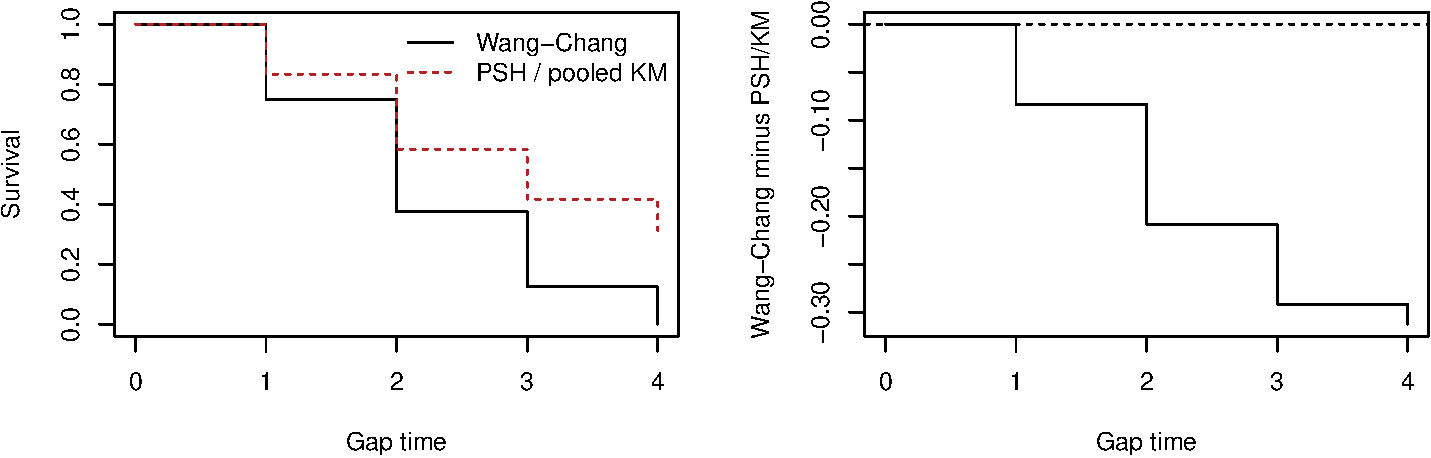
\includegraphics[keepaspectratio]{jss-manuscript_files/figure-pdf/fig-curves-1.pdf}}

}

\caption{\label{fig-curves}Wang--Chang and PSH/pooled Kaplan--Meier
survival on the example records, and their difference.}

\end{figure}%

\subsection{Rank tests and paired
visits}\label{rank-tests-and-paired-visits}

\texttt{wc\_logrank()} implements the two-group Luo--Huang
weighted-risk-set \citep{luo2011} \(G_\rho^*\) statistic. At each event
time it contrasts weighted observed events with their group-specific
weighted risk-set expectation. With \(\rho=0\), it is the recurrent
gap-time log-rank analogue; \(\rho=1\) gives a Peto--Prentice-type
weight. The variance is based on subject-level martingale-style
contributions to retain within-subject gap dependence.

\texttt{zhao\_rank\_test()} is separate. It implements the extended LR,
Gehan--Breslow, and Peto--Prentice score construction described by
\citet{zhao2020}. Its default \texttt{pooled\_risk} residual is assessed
by the simulations below; current results do not establish
published-table reproduction. The group-risk denominator printed in Zhao
et al.'s Equation 6 is retained as the explicit \texttt{zhao\_eq6}
sensitivity/reproduction path. Neither function should be described as
an exact substitute for the other.

For two paired visits per participant,
\texttt{wc\_paired\_permutation()} swaps labels within participant pairs
and recalculates \(G_\rho^*\). Its p-value tests the within-pair
label-exchangeability null. The independent-arm analytical p-value from
\texttt{wc\_logrank()} is returned for context but is not a paired
analysis.

\subsection{Recurrent competing risks}\label{recurrent-competing-risks}

\texttt{ss\_rcif()} implements recurrent cause-specific
cumulative-incidence functions following \citet{sivadasan2023}. The
default shared weighting keeps pooled and cause-specific increments
additive. \texttt{cause\_weighting\ =\ "literal\_eq15"} is retained as a
sensitivity/reproduction option because literal use of the printed
Equation 15 denominator can yield nonadditive increments.

\texttt{ss\_rcif\_equal\_causes\_test()} is a subject-bootstrap Wald
reconstruction of the METRON equal-cause test \citep{sisuma2022}. It
compares integrated RCIF contrasts and must not be called a log-rank
test.

\subsection{Validation against prior
implementations}\label{validation-against-prior-implementations}

The following checks rerun the continuous-data examples from the
reference vignettes with fixed seeds. Each row compares the same
event-time grid and survival values with the indicated installed package
\citep{survrec, newtestsurvrec}. Optional packages are not downloaded
during rendering; missing installations produce an explicit unavailable
result. The package versions and discrepancies are computed at render
time, not copied from previous output.

\begin{Shaded}
\begin{Highlighting}[]
\NormalTok{reference\_checks }\OtherTok{\textless{}{-}} \FunctionTok{manuscript\_reference\_checks}\NormalTok{()}
\NormalTok{reference\_display }\OtherTok{\textless{}{-}}\NormalTok{ reference\_checks}
\NormalTok{reference\_display}\SpecialCharTok{$}\NormalTok{Max\_absolute\_difference }\OtherTok{\textless{}{-}} \FunctionTok{ifelse}\NormalTok{(}
  \FunctionTok{is.na}\NormalTok{(reference\_checks}\SpecialCharTok{$}\NormalTok{Max\_absolute\_difference), }\StringTok{"Not run"}\NormalTok{,}
  \FunctionTok{formatC}\NormalTok{(reference\_checks}\SpecialCharTok{$}\NormalTok{Max\_absolute\_difference, }\AttributeTok{format =} \StringTok{"e"}\NormalTok{, }\AttributeTok{digits =} \DecValTok{3}\NormalTok{))}
\NormalTok{knitr}\SpecialCharTok{::}\FunctionTok{kable}\NormalTok{(reference\_display)}
\end{Highlighting}
\end{Shaded}

{

\begin{longtable}[]{@{}
  >{\raggedright\arraybackslash}p{(\linewidth - 8\tabcolsep) * \real{0.3049}}
  >{\raggedright\arraybackslash}p{(\linewidth - 8\tabcolsep) * \real{0.1220}}
  >{\raggedright\arraybackslash}p{(\linewidth - 8\tabcolsep) * \real{0.1829}}
  >{\raggedright\arraybackslash}p{(\linewidth - 8\tabcolsep) * \real{0.0976}}
  >{\raggedright\arraybackslash}p{(\linewidth - 8\tabcolsep) * \real{0.2927}}@{}}

\caption{\label{tbl-reference-checks}Numerical comparisons for
Wang--Chang and PSH estimators. Missing differences indicate an
unavailable reference package.}

\tabularnewline

\toprule\noalign{}
\begin{minipage}[b]{\linewidth}\raggedright
Scenario
\end{minipage} & \begin{minipage}[b]{\linewidth}\raggedright
Estimator
\end{minipage} & \begin{minipage}[b]{\linewidth}\raggedright
Reference
\end{minipage} & \begin{minipage}[b]{\linewidth}\raggedright
Version
\end{minipage} & \begin{minipage}[b]{\linewidth}\raggedright
Max\_absolute\_difference
\end{minipage} \\
\midrule\noalign{}
\endhead
\bottomrule\noalign{}
\endlastfoot
100 subjects, 1-5 events & WC & survrec & 1.2.5 & 1.055e-15 \\
100 subjects, 1-5 events & WC & newTestSurvRec & 1.0.2 & 3.333e-09 \\
100 subjects, 1-5 events & PSH & survrec & 1.2.5 & 0.000e+00 \\
100 subjects, 1-5 events & PSH & newTestSurvRec & 1.0.2 & 0.000e+00 \\
80 subjects, 0-6 events & WC & survrec & 1.2.5 & 5.551e-17 \\
80 subjects, 0-6 events & WC & newTestSurvRec & 1.0.2 & 4.999e-09 \\
80 subjects, 0-6 events & PSH & survrec & 1.2.5 & 0.000e+00 \\
80 subjects, 0-6 events & PSH & newTestSurvRec & 1.0.2 & 0.000e+00 \\

\end{longtable}

}

These are software comparisons for the estimators of \citet{wang1999}
and \citet{pena2001}. They are not reproductions of the simulation
tables in those papers. In particular, \texttt{newTestSurvRec}'s
\texttt{LRrec} pathway is associated with PSH-style estimation and is
not a numerical reference for the Luo--Huang rank test.

\begin{Shaded}
\begin{Highlighting}[]
\NormalTok{rank\_example }\OtherTok{\textless{}{-}} \FunctionTok{do.call}\NormalTok{(rbind, }\FunctionTok{lapply}\NormalTok{(}\FunctionTok{c}\NormalTok{(}\DecValTok{0}\NormalTok{, }\DecValTok{1}\NormalTok{), }\ControlFlowTok{function}\NormalTok{(rho) \{}
\NormalTok{  fit }\OtherTok{\textless{}{-}} \FunctionTok{wc\_logrank}\NormalTok{(gaps, }\AttributeTok{group =} \StringTok{"arm"}\NormalTok{, }\AttributeTok{episode =} \StringTok{"episode"}\NormalTok{, }\AttributeTok{rho =}\NormalTok{ rho)}
  \FunctionTok{data.frame}\NormalTok{(}\AttributeTok{Method =} \FunctionTok{paste0}\NormalTok{(}\StringTok{"Luo{-}Huang, rho = "}\NormalTok{, rho),}
             \AttributeTok{z =}\NormalTok{ fit}\SpecialCharTok{$}\NormalTok{z, }\AttributeTok{p\_value =}\NormalTok{ fit}\SpecialCharTok{$}\NormalTok{p.value)}
\NormalTok{\}))}
\NormalTok{knitr}\SpecialCharTok{::}\FunctionTok{kable}\NormalTok{(rank\_example, }\AttributeTok{digits =} \DecValTok{4}\NormalTok{)}
\end{Highlighting}
\end{Shaded}

{

\begin{longtable}[]{@{}lrr@{}}

\caption{\label{tbl-rank-example}Executable rank-test example on the
four-subject illustration. These values demonstrate the interface and
are not simulation validation.}

\tabularnewline

\toprule\noalign{}
Method & z & p\_value \\
\midrule\noalign{}
\endhead
\bottomrule\noalign{}
\endlastfoot
Luo-Huang, rho = 0 & 1.9612 & 0.0499 \\
Luo-Huang, rho = 1 & 1.7598 & 0.0784 \\

\end{longtable}

}

\textbf{Published-benchmark placeholder for Wang--Chang and Luo--Huang.}
The curve in Figure~\ref{fig-curves}, the independent pooled-KM check,
and Table~\ref{tbl-reference-checks} provide reproducible estimator
checks. Direct numerical reproduction of the original Wang--Chang and
Luo--Huang simulation tables \citep{wang1999, luo2011} remains a
separate validation task requiring a matched design and transcribed
published benchmarks. Zhao's results below assess a different rank-test
construction and cannot fill that role. The existing K-group PSG
simulation is an application-specific extension check, not a
reproduction of Luo--Huang's two-group study.

\subsection{Simulation validation}\label{simulation-validation}

\subsubsection{Zhao published-table
comparison}\label{sec-zhao-validation}

This section compares completed runs with the \textbf{New method}
columns of Tables 1--3 in \citet{zhao2020}. Table 1 reports the SD of
the standardized null statistic; Table 2 reports one-sided type-I error
at \(\alpha=0.025\); Table 3 reports power. LR, PP, and GB denote
log-rank, Peto--Prentice, and Gehan--Breslow weights. OLR and
Jung--Jeong columns are not used as benchmarks for this implementation.

\texttt{data-raw/zhao-2020-table-simulations.R} defines 120 cells with
four baseline distributions, three heterogeneity ranges, 100 subjects
per arm, study end 180 days, and entry uniform on \((0,180)\). Subject
gap multipliers follow \(Z\sim U(0.5,1.5)\), \(U(0.1,1.9)\), or
\(U(0.01,1.99)\), labeled low, medium, and high heterogeneity. The
intended numbers of simulated datasets are 100,000 per null cell and
10,000 per power cell. Treatment gaps in Table 3 are multiplied by
\(\exp(0.25)\) or \(\exp(0.5)\); for Weibull shape 2 these correspond to
changes of 0.5 and 1 in \(-\log(\lambda)\).

The baseline laws in the corrected generator match Table 1: exponential
rate \(\exp(-4)\), Weibull shape 2 and scale \(\exp(4)\), log-normal
parameters \((\mu,\sigma)=(4,0.5)\), and log-logistic survival
\(S(t)=\{1+[\exp(-4)t]^2\}^{-1}\). The local generator uses
administrative censoring. Zhao used \texttt{survsim::rec.ev.surv()}
\citep{survsim} and discussed an additional noninformative censoring
mechanism without full parameter details in Section 3. Thus matching
baseline distributions does not establish identical simulation designs.

The reference CSV, \texttt{data-raw/zhao-2020-published-tables.csv}, was
transcribed from pages 93--95 of the publisher PDF. \textbf{Table 2 has
a scale ambiguity:} its caption says ``(*100)'' but prints integers such
as 27 and 25. We interpret these as 0.027 and 0.025, consistent with
Section 3.2's nominal 0.025 level and interpretation. This is an
explicit, unconfirmed correction; both raw printed values and
interpreted probabilities are retained. Table 2 comparisons are
conditional on it.

\begin{Shaded}
\begin{Highlighting}[]
\NormalTok{zhao }\OtherTok{\textless{}{-}} \FunctionTok{manuscript\_zhao}\NormalTok{(repo\_root)}
\NormalTok{zhao\_status }\OtherTok{\textless{}{-}} \FunctionTok{manuscript\_zhao\_status}\NormalTok{(zhao)}
\NormalTok{zhao\_available }\OtherTok{\textless{}{-}} \FunctionTok{sum}\NormalTok{(zhao}\SpecialCharTok{$}\NormalTok{available)}
\NormalTok{zhao\_comparable }\OtherTok{\textless{}{-}} \FunctionTok{sum}\NormalTok{(zhao}\SpecialCharTok{$}\NormalTok{available }\SpecialCharTok{\&}\NormalTok{ zhao}\SpecialCharTok{$}\NormalTok{design\_eligible)}
\NormalTok{zhao\_discrepant }\OtherTok{\textless{}{-}} \FunctionTok{sum}\NormalTok{(zhao}\SpecialCharTok{$}\NormalTok{comparison }\SpecialCharTok{==} \StringTok{"discrepant"}\NormalTok{)}
\NormalTok{zhao\_method }\OtherTok{\textless{}{-}} \ControlFlowTok{if}\NormalTok{ (zhao\_available) }\FunctionTok{unique}\NormalTok{(zhao}\SpecialCharTok{$}\NormalTok{variance\_method) }\ControlFlowTok{else} \StringTok{"not available"}
\end{Highlighting}
\end{Shaded}

At this render, \textbf{86 of 120 cells} are available, of which 86
satisfy the recorded design-eligibility checks. The variance convention
recorded in these files is \textbf{pooled\_risk}. Availability is
assessed from files, not scheduler status. Missing files are shown as
\emph{Pending}; they do not contribute zero rejection rates or enter
comparison summaries. \texttt{pooled\_risk} and the printed Equation 6
group-risk convention (\texttt{zhao\_eq6}) remain distinct; the importer
rejects mixtures of variance conventions and inconsistent settings. The
\texttt{zhao\_eq6} comparison remains pending unless a separate,
consistently configured result directory is supplied.

\begin{Shaded}
\begin{Highlighting}[]
\NormalTok{knitr}\SpecialCharTok{::}\FunctionTok{kable}\NormalTok{(zhao\_status)}
\end{Highlighting}
\end{Shaded}

{

\begin{longtable}[]{@{}
  >{\raggedright\arraybackslash}p{(\linewidth - 14\tabcolsep) * \real{0.0645}}
  >{\raggedleft\arraybackslash}p{(\linewidth - 14\tabcolsep) * \real{0.0860}}
  >{\raggedleft\arraybackslash}p{(\linewidth - 14\tabcolsep) * \real{0.1075}}
  >{\raggedleft\arraybackslash}p{(\linewidth - 14\tabcolsep) * \real{0.1183}}
  >{\raggedleft\arraybackslash}p{(\linewidth - 14\tabcolsep) * \real{0.0860}}
  >{\raggedleft\arraybackslash}p{(\linewidth - 14\tabcolsep) * \real{0.0968}}
  >{\raggedright\arraybackslash}p{(\linewidth - 14\tabcolsep) * \real{0.3226}}
  >{\raggedleft\arraybackslash}p{(\linewidth - 14\tabcolsep) * \real{0.1183}}@{}}

\caption{\label{tbl-zhao-completeness}Available and missing cells in the
Zhao validation design. Discrepant counts use the exploratory Monte
Carlo criterion below.}

\tabularnewline

\toprule\noalign{}
\begin{minipage}[b]{\linewidth}\raggedright
Table
\end{minipage} & \begin{minipage}[b]{\linewidth}\raggedleft
Planned
\end{minipage} & \begin{minipage}[b]{\linewidth}\raggedleft
Available
\end{minipage} & \begin{minipage}[b]{\linewidth}\raggedleft
Comparable
\end{minipage} & \begin{minipage}[b]{\linewidth}\raggedleft
Missing
\end{minipage} & \begin{minipage}[b]{\linewidth}\raggedleft
Excluded
\end{minipage} & \begin{minipage}[b]{\linewidth}\raggedright
Replicates\_per\_available\_cell
\end{minipage} & \begin{minipage}[b]{\linewidth}\raggedleft
Discrepant
\end{minipage} \\
\midrule\noalign{}
\endhead
\bottomrule\noalign{}
\endlastfoot
1 & 12 & 9 & 9 & 3 & 0 & 100000 & 3 \\
2 & 36 & 24 & 24 & 12 & 0 & 100000 & 4 \\
3 & 72 & 53 & 53 & 19 & 0 & 10000 & 53 \\

\end{longtable}

}

An earlier log-logistic generator used an incorrect scale and inverse
transform, producing vastly too many recurrences. Those outputs cannot
validate Zhao's design. Corrected runs carry
\texttt{generator\_version\ =\ "zhao\_table1\_loglogistic\_v2"}; legacy
log-logistic outputs are displayed as \emph{Excluded}. Existing results
for the other three distributions are retained. Rerendering
automatically incorporates newly completed, eligible cells, including
all 120 when available.

\paragraph{Monte Carlo uncertainty and current
findings}\label{monte-carlo-uncertainty-and-current-findings}

For a rejection proportion \(\hat p\) based on \(B\) replicates, the
Monte Carlo standard error is \(\{\hat p(1-\hat p)/B\}^{1/2}\). Local
rejection-rate intervals use Wilson's formula. For empirical SDs in
Table 1 we use the normal-theory approximation
\(\operatorname{MCSE}(s)=s/\sqrt{2(B-1)}\); replicate-level fourth
moments are unavailable, so this is approximate. A cell receives an
asterisk when

\[
|\widehat\theta_{\mathrm{local}}-\widehat\theta_{\mathrm{paper}}|
>1.96\sqrt{\operatorname{MCSE}_{\mathrm{local}}^2+
             \operatorname{MCSE}_{\mathrm{paper}}^2}+0.0005.
\]

The last term allows half a unit of rounding in the published tables.
The calculation assumes independent simulation runs and uses the paper's
replicate counts. It is an exploratory cellwise discrepancy screen, not
an equivalence test or a multiplicity-adjusted global validation rule. A
cell without an asterisk is not proven equivalent. Nominal calibration
is assessed separately in the exported CSV by exact binomial tests
against 0.025, with Holm adjustment across the 36 planned Table 2 cells.

Among the 86 comparable completed cells, \textbf{60 are discrepant}
under the criterion above.

Across 53 available power cells, local minus published power ranges from
\textbf{+0.46 to +33.44 percentage points}. These results require
investigation of the generator/censoring design and variance convention
before claiming published-table reproduction.

The original RDS files retain summary moments, not individual simulated
statistics or failed-p-value counts. Consequently, the null histogram in
Zhao's Figure 1 cannot be reconstructed from this batch. No histogram is
inferred from a mean and SD. The figure below instead compares the
reported quantities directly, while the following three tables retain
the distribution, heterogeneity, alternative, and LR/PP/GB arrangement
of Zhao's tables.

\begin{Shaded}
\begin{Highlighting}[]
\FunctionTok{manuscript\_zhao\_plot}\NormalTok{(zhao)}
\end{Highlighting}
\end{Shaded}

\begin{figure}[H]

\centering{

\pandocbounded{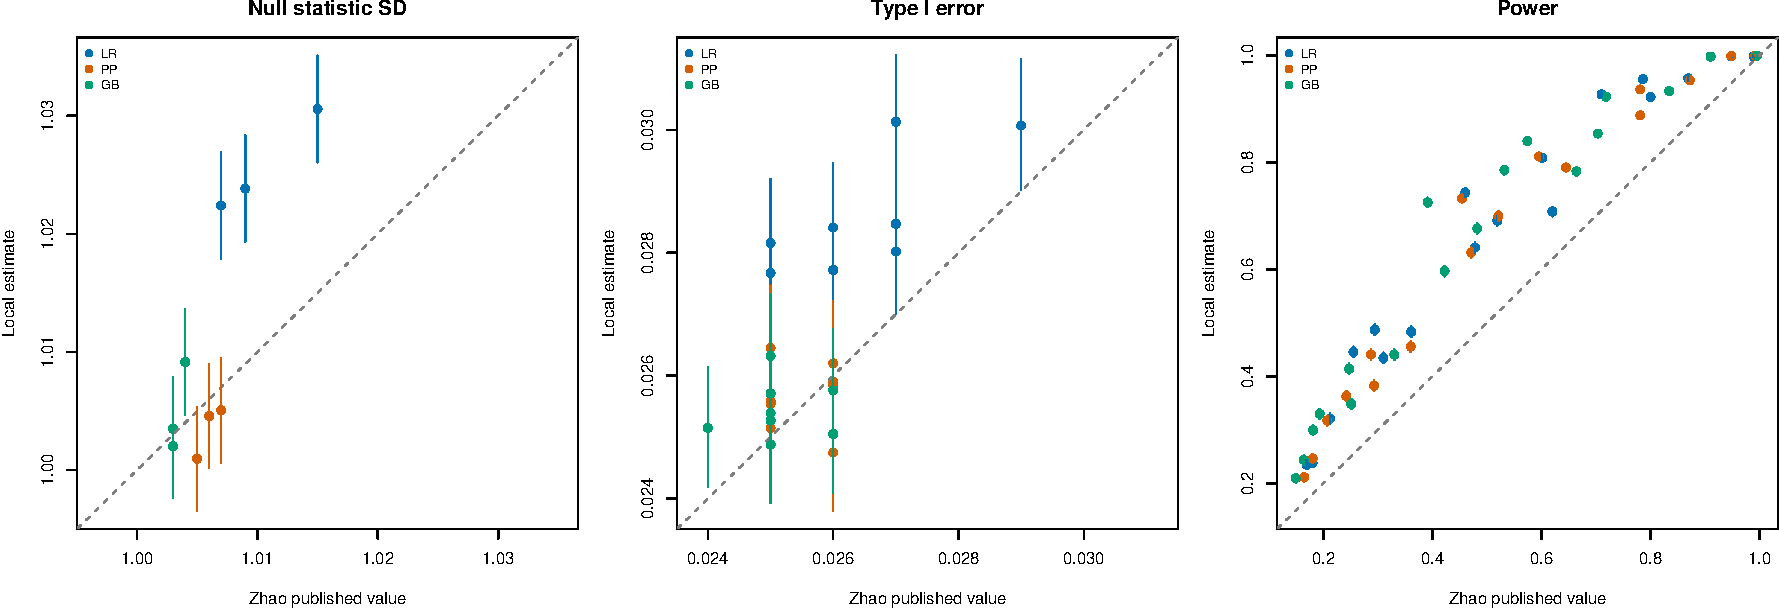
\includegraphics[keepaspectratio]{jss-manuscript_files/figure-pdf/fig-zhao-comparison-1.pdf}}

}

\caption{\label{fig-zhao-comparison}Published versus local Zhao
simulation summaries. The dashed line is equality. Bars show local 95\%
Monte Carlo intervals (normal approximation for SDs, Wilson intervals
for rejection rates). Paper uncertainty and rounding also enter the
discrepancy screen. Only available, design-eligible cells are plotted.}

\end{figure}%

\begin{Shaded}
\begin{Highlighting}[]
\NormalTok{knitr}\SpecialCharTok{::}\FunctionTok{kable}\NormalTok{(}\FunctionTok{manuscript\_zhao\_table}\NormalTok{(zhao, }\StringTok{"table1"}\NormalTok{))}
\end{Highlighting}
\end{Shaded}

{

\begin{longtable}[]{@{}
  >{\raggedright\arraybackslash}p{(\linewidth - 12\tabcolsep) * \real{0.1494}}
  >{\raggedright\arraybackslash}p{(\linewidth - 12\tabcolsep) * \real{0.0920}}
  >{\raggedright\arraybackslash}p{(\linewidth - 12\tabcolsep) * \real{0.2069}}
  >{\raggedright\arraybackslash}p{(\linewidth - 12\tabcolsep) * \real{0.0920}}
  >{\raggedright\arraybackslash}p{(\linewidth - 12\tabcolsep) * \real{0.1839}}
  >{\raggedright\arraybackslash}p{(\linewidth - 12\tabcolsep) * \real{0.0920}}
  >{\raggedright\arraybackslash}p{(\linewidth - 12\tabcolsep) * \real{0.1839}}@{}}

\caption{\label{tbl-zhao-null-sd}Comparison with Zhao Table 1: empirical
SD of the standardized null statistic at medium heterogeneity.
Parentheses contain local Monte Carlo SEs; an asterisk marks a
discrepancy.}

\tabularnewline

\toprule\noalign{}
\begin{minipage}[b]{\linewidth}\raggedright
Distribution
\end{minipage} & \begin{minipage}[b]{\linewidth}\raggedright
LR Zhao
\end{minipage} & \begin{minipage}[b]{\linewidth}\raggedright
LR local (MCSE)
\end{minipage} & \begin{minipage}[b]{\linewidth}\raggedright
PP Zhao
\end{minipage} & \begin{minipage}[b]{\linewidth}\raggedright
PP local (MCSE)
\end{minipage} & \begin{minipage}[b]{\linewidth}\raggedright
GB Zhao
\end{minipage} & \begin{minipage}[b]{\linewidth}\raggedright
GB local (MCSE)
\end{minipage} \\
\midrule\noalign{}
\endhead
\bottomrule\noalign{}
\endlastfoot
exponential & 1.007 & 1.0224 (0.0023) * & 1.005 & 1.0010 (0.0022) &
1.004 & 1.0092 (0.0023) \\
weibull & 1.015 & 1.0306 (0.0023) * & 1.007 & 1.0051 (0.0022) & 1.003 &
1.0035 (0.0022) \\
lognormal & 1.009 & 1.0238 (0.0023) * & 1.006 & 1.0046 (0.0022) & 1.003
& 1.0020 (0.0022) \\
loglogistic & 1.009 & Pending & 0.997 & Pending & 0.998 & Pending \\

\end{longtable}

}

\begin{Shaded}
\begin{Highlighting}[]
\NormalTok{knitr}\SpecialCharTok{::}\FunctionTok{kable}\NormalTok{(}\FunctionTok{manuscript\_zhao\_table}\NormalTok{(zhao, }\StringTok{"table2"}\NormalTok{))}
\end{Highlighting}
\end{Shaded}

{

\begin{longtable}[]{@{}
  >{\raggedright\arraybackslash}p{(\linewidth - 14\tabcolsep) * \real{0.1386}}
  >{\raggedright\arraybackslash}p{(\linewidth - 14\tabcolsep) * \real{0.1287}}
  >{\raggedright\arraybackslash}p{(\linewidth - 14\tabcolsep) * \real{0.0792}}
  >{\raggedright\arraybackslash}p{(\linewidth - 14\tabcolsep) * \real{0.1782}}
  >{\raggedright\arraybackslash}p{(\linewidth - 14\tabcolsep) * \real{0.0792}}
  >{\raggedright\arraybackslash}p{(\linewidth - 14\tabcolsep) * \real{0.1584}}
  >{\raggedright\arraybackslash}p{(\linewidth - 14\tabcolsep) * \real{0.0792}}
  >{\raggedright\arraybackslash}p{(\linewidth - 14\tabcolsep) * \real{0.1584}}@{}}

\caption{\label{tbl-zhao-type1}Comparison with Zhao Table 2: one-sided
type-I error probabilities. Published integers are divided by 1000 as
explained in the text. Parentheses contain local Monte Carlo SEs; an
asterisk marks a discrepancy.}

\tabularnewline

\toprule\noalign{}
\begin{minipage}[b]{\linewidth}\raggedright
Heterogeneity
\end{minipage} & \begin{minipage}[b]{\linewidth}\raggedright
Distribution
\end{minipage} & \begin{minipage}[b]{\linewidth}\raggedright
LR Zhao
\end{minipage} & \begin{minipage}[b]{\linewidth}\raggedright
LR local (MCSE)
\end{minipage} & \begin{minipage}[b]{\linewidth}\raggedright
PP Zhao
\end{minipage} & \begin{minipage}[b]{\linewidth}\raggedright
PP local (MCSE)
\end{minipage} & \begin{minipage}[b]{\linewidth}\raggedright
GB Zhao
\end{minipage} & \begin{minipage}[b]{\linewidth}\raggedright
GB local (MCSE)
\end{minipage} \\
\midrule\noalign{}
\endhead
\bottomrule\noalign{}
\endlastfoot
low & exponential & 0.027 & 0.0280 (0.0005) & 0.026 & 0.0262 (0.0005) &
0.026 & Pending \\
low & weibull & 0.029 & 0.0301 (0.0005) & 0.026 & 0.0259 (0.0005) &
0.025 & 0.0254 (0.0005) \\
low & lognormal & 0.027 & 0.0301 (0.0005) * & 0.025 & 0.0265 (0.0005) &
0.026 & 0.0250 (0.0005) \\
low & loglogistic & 0.026 & Pending & 0.026 & Pending & 0.025 &
Pending \\
medium & exponential & 0.026 & 0.0284 (0.0005) * & 0.025 & 0.0255
(0.0005) & 0.026 & 0.0258 (0.0005) \\
medium & weibull & 0.027 & 0.0285 (0.0005) & 0.026 & 0.0259 (0.0005) &
0.025 & 0.0263 (0.0005) \\
medium & lognormal & 0.025 & 0.0277 (0.0005) * & 0.025 & 0.0251 (0.0005)
& 0.025 & 0.0257 (0.0005) \\
medium & loglogistic & 0.026 & Pending & 0.025 & Pending & 0.025 &
Pending \\
high & exponential & 0.026 & Pending & 0.026 & Pending & 0.025 & 0.0249
(0.0005) \\
high & weibull & 0.025 & 0.0282 (0.0005) * & 0.025 & 0.0256 (0.0005) &
0.024 & 0.0251 (0.0005) \\
high & lognormal & 0.026 & 0.0277 (0.0005) & 0.026 & 0.0248 (0.0005) &
0.025 & 0.0253 (0.0005) \\
high & loglogistic & 0.025 & Pending & 0.025 & Pending & 0.024 &
Pending \\

\end{longtable}

}

\begin{Shaded}
\begin{Highlighting}[]
\NormalTok{knitr}\SpecialCharTok{::}\FunctionTok{kable}\NormalTok{(}\FunctionTok{manuscript\_zhao\_table}\NormalTok{(zhao, }\StringTok{"table3"}\NormalTok{))}
\end{Highlighting}
\end{Shaded}

{

\begin{longtable}[]{@{}
  >{\raggedright\arraybackslash}p{(\linewidth - 16\tabcolsep) * \real{0.1167}}
  >{\raggedright\arraybackslash}p{(\linewidth - 16\tabcolsep) * \real{0.1083}}
  >{\raggedleft\arraybackslash}p{(\linewidth - 16\tabcolsep) * \real{0.1250}}
  >{\raggedright\arraybackslash}p{(\linewidth - 16\tabcolsep) * \real{0.0667}}
  >{\raggedright\arraybackslash}p{(\linewidth - 16\tabcolsep) * \real{0.1500}}
  >{\raggedright\arraybackslash}p{(\linewidth - 16\tabcolsep) * \real{0.0667}}
  >{\raggedright\arraybackslash}p{(\linewidth - 16\tabcolsep) * \real{0.1500}}
  >{\raggedright\arraybackslash}p{(\linewidth - 16\tabcolsep) * \real{0.0667}}
  >{\raggedright\arraybackslash}p{(\linewidth - 16\tabcolsep) * \real{0.1500}}@{}}

\caption{\label{tbl-zhao-power}Comparison with Zhao Table 3: one-sided
power probabilities. Parentheses contain local Monte Carlo SEs; an
asterisk marks a discrepancy. The log-time shift is 0.25 or 0.5 for all
four distributions.}

\tabularnewline

\toprule\noalign{}
\begin{minipage}[b]{\linewidth}\raggedright
Heterogeneity
\end{minipage} & \begin{minipage}[b]{\linewidth}\raggedright
Distribution
\end{minipage} & \begin{minipage}[b]{\linewidth}\raggedleft
Log-time shift
\end{minipage} & \begin{minipage}[b]{\linewidth}\raggedright
LR Zhao
\end{minipage} & \begin{minipage}[b]{\linewidth}\raggedright
LR local (MCSE)
\end{minipage} & \begin{minipage}[b]{\linewidth}\raggedright
PP Zhao
\end{minipage} & \begin{minipage}[b]{\linewidth}\raggedright
PP local (MCSE)
\end{minipage} & \begin{minipage}[b]{\linewidth}\raggedright
GB Zhao
\end{minipage} & \begin{minipage}[b]{\linewidth}\raggedright
GB local (MCSE)
\end{minipage} \\
\midrule\noalign{}
\endhead
\bottomrule\noalign{}
\endlastfoot
low & exponential & 0.25 & 0.212 & 0.3209 (0.0047) * & 0.207 & 0.3172
(0.0047) * & 0.181 & 0.2994 (0.0046) * \\
low & exponential & 0.50 & 0.601 & 0.8085 (0.0039) * & 0.595 & 0.8111
(0.0039) * & 0.532 & 0.7858 (0.0041) * \\
low & weibull & 0.25 & 0.460 & 0.7437 (0.0044) * & 0.454 & 0.7326
(0.0044) * & 0.391 & 0.7254 (0.0045) * \\
low & weibull & 0.50 & 0.948 & 0.9985 (0.0004) * & 0.948 & 0.9990
(0.0003) * & 0.910 & 0.9980 (0.0004) * \\
low & lognormal & 0.25 & 0.620 & 0.7083 (0.0045) * & 0.645 & 0.7904
(0.0041) * & 0.664 & 0.7836 (0.0041) * \\
low & lognormal & 0.50 & 0.989 & 0.9982 (0.0004) * & 0.992 & 0.9996
(0.0002) * & 0.995 & 0.9996 (0.0002) * \\
low & loglogistic & 0.25 & 0.325 & Pending & 0.334 & Pending & 0.334 &
Pending \\
low & loglogistic & 0.50 & 0.828 & Pending & 0.846 & Pending & 0.852 &
Pending \\
medium & exponential & 0.25 & 0.180 & 0.2384 (0.0043) * & 0.180 & 0.2462
(0.0043) * & 0.164 & 0.2438 (0.0043) * \\
medium & exponential & 0.50 & 0.519 & 0.6914 (0.0046) * & 0.521 & 0.6996
(0.0046) * & 0.482 & 0.6765 (0.0047) * \\
medium & weibull & 0.25 & 0.294 & 0.4871 (0.0050) * & 0.287 & 0.4410
(0.0050) * & 0.247 & 0.4140 (0.0049) * \\
medium & weibull & 0.50 & 0.786 & 0.9560 (0.0021) * & 0.781 & 0.9365
(0.0024) * & 0.718 & 0.9230 (0.0027) * \\
medium & lognormal & 0.25 & 0.361 & 0.4834 (0.0050) * & 0.360 & 0.4557
(0.0050) * & 0.330 & 0.4405 (0.0050) * \\
medium & lognormal & 0.50 & 0.869 & 0.9573 (0.0020) * & 0.872 & 0.9537
(0.0021) * & 0.834 & 0.9335 (0.0025) * \\
medium & loglogistic & 0.25 & 0.242 & Pending & 0.247 & Pending & 0.230
& Pending \\
medium & loglogistic & 0.50 & 0.695 & Pending & 0.711 & Pending & 0.688
& Pending \\
high & exponential & 0.25 & 0.169 & 0.2347 (0.0042) * & 0.165 & 0.2114
(0.0041) * & 0.149 & 0.2096 (0.0041) * \\
high & exponential & 0.50 & 0.478 & 0.6408 (0.0048) * & 0.471 & 0.6316
(0.0048) * & 0.422 & 0.5967 (0.0049) * \\
high & weibull & 0.25 & 0.255 & 0.4456 (0.0050) * & 0.242 & 0.3630
(0.0048) * & 0.193 & 0.3300 (0.0047) * \\
high & weibull & 0.50 & 0.710 & 0.9273 (0.0026) * & 0.683 & Pending &
0.574 & 0.8399 (0.0037) * \\
high & lognormal & 0.25 & 0.310 & 0.4345 (0.0050) * & 0.293 & 0.3825
(0.0049) * & 0.251 & 0.3481 (0.0048) * \\
high & lognormal & 0.50 & 0.800 & 0.9223 (0.0027) * & 0.781 & 0.8880
(0.0032) * & 0.703 & 0.8541 (0.0035) * \\
high & loglogistic & 0.25 & 0.210 & Pending & 0.212 & Pending & 0.191 &
Pending \\
high & loglogistic & 0.50 & 0.614 & Pending & 0.617 & Pending & 0.569 &
Pending \\

\end{longtable}

}

\textbf{Full-run placeholder.} These same chunks will produce the
full-data tables and plot after the remaining RDS files are copied into
the input directory. Rendering never starts the 100,000-replicate jobs.
Use a separate directory and \texttt{ZHAO\_RESULTS\_DIR} to render a
different variance convention rather than pooling results across
methods. The completed-cell findings above remain provisional until the
design differences and observed discrepancies are resolved.

\subsubsection{PSG-shaped simulation
study}\label{psg-shaped-simulation-study}

The PSG supplement script simulates recurrent bouts with: (i) subject
frailty, (ii) visit effects, (iii) persistent burst/recovery states,
(iv) 360--480 minute recordings with terminal censoring, (v) unequal
independent-arm sizes (30 control, 45 treatment), and (vi) paired visits
with shared participant frailty. Under the null, treatment and control
gaps have the same distribution. Power alternatives multiply treatment
gaps by 1.25 (longer bouts) or 0.80 (shorter bouts). The script
evaluates \(G_0^*\), \(G_1^*\), Zhao pooled-risk sensitivity analyses,
and paired label permutations where appropriate.

\begin{Shaded}
\begin{Highlighting}[]
\NormalTok{psg\_file }\OtherTok{\textless{}{-}} \FunctionTok{Sys.getenv}\NormalTok{(}\StringTok{"PSG\_RESULTS\_FILE"}\NormalTok{, }\FunctionTok{file.path}\NormalTok{(repo\_root, }\StringTok{"data{-}raw/psg{-}validation{-}results.rds"}\NormalTok{))}
\ControlFlowTok{if}\NormalTok{ (}\SpecialCharTok{!}\FunctionTok{grepl}\NormalTok{(}\StringTok{"\^{}(/|[A{-}Za{-}z]:)"}\NormalTok{, psg\_file)) psg\_file }\OtherTok{\textless{}{-}} \FunctionTok{file.path}\NormalTok{(repo\_root, psg\_file)}
\ControlFlowTok{if}\NormalTok{ (}\FunctionTok{file.exists}\NormalTok{(psg\_file)) \{}
\NormalTok{  psg\_results }\OtherTok{\textless{}{-}} \FunctionTok{readRDS}\NormalTok{(psg\_file)}
  \FunctionTok{stopifnot}\NormalTok{(}\FunctionTok{is.data.frame}\NormalTok{(psg\_results),}
    \FunctionTok{all}\NormalTok{(}\FunctionTok{c}\NormalTok{(}\StringTok{"design"}\NormalTok{, }\StringTok{"alternative"}\NormalTok{, }\StringTok{"method"}\NormalTok{, }\StringTok{"n\_sim"}\NormalTok{, }\StringTok{"B"}\NormalTok{, }\StringTok{"rejection\_rate"}\NormalTok{, }\StringTok{"monte\_carlo\_se"}\NormalTok{) }\SpecialCharTok{\%in\%} \FunctionTok{names}\NormalTok{(psg\_results)))}
  \FunctionTok{cat}\NormalTok{(}\StringTok{"Available PSG summaries are shown with their actual replicate and permutation counts; small runs are pilots, not full{-}study validation.}\SpecialCharTok{\textbackslash{}n\textbackslash{}n}\StringTok{"}\NormalTok{)}
  \FunctionTok{print}\NormalTok{(knitr}\SpecialCharTok{::}\FunctionTok{kable}\NormalTok{(psg\_results, }\AttributeTok{digits =} \DecValTok{4}\NormalTok{))}
\NormalTok{\} }\ControlFlowTok{else}\NormalTok{ \{}
  \FunctionTok{cat}\NormalTok{(}\StringTok{"**Results placeholder.** No combined PSG result file is available. The planned 1,000{-}replicate/999{-}permutation results will be imported on rerender when \textasciigrave{}data{-}raw/psg{-}validation{-}results.rds\textasciigrave{} is supplied. Set \textasciigrave{}PSG\_RESULTS\_FILE\textasciigrave{} to select a different result file.}\SpecialCharTok{\textbackslash{}n\textbackslash{}n}\StringTok{"}\NormalTok{)}
\NormalTok{\}}
\end{Highlighting}
\end{Shaded}

\textbf{Results placeholder.} No combined PSG result file is available.
The planned 1,000-replicate/999-permutation results will be imported on
rerender when \texttt{data-raw/psg-validation-results.rds} is supplied.
Set \texttt{PSG\_RESULTS\_FILE} to select a different result file.

\subsubsection{K-group application-specific
pilot}\label{k-group-application-specific-pilot}

The following table imports the existing K-group output, if available.
Its replicate count is displayed explicitly. It assesses the package's
extension of the weighted-risk-set score to three unequal arms under the
PSG-shaped design in
\texttt{data-raw/wc-logrank-k-validation-simulation.R}. It is not a
published numerical benchmark from \citet{luo2011}, and a small pilot
does not establish type-I-error control.

\begin{Shaded}
\begin{Highlighting}[]
\NormalTok{k\_file }\OtherTok{\textless{}{-}} \FunctionTok{file.path}\NormalTok{(repo\_root, }\StringTok{"data{-}raw/wc{-}logrank{-}k{-}validation{-}results.csv"}\NormalTok{)}
\ControlFlowTok{if}\NormalTok{ (}\FunctionTok{file.exists}\NormalTok{(k\_file)) \{}
\NormalTok{  k\_results }\OtherTok{\textless{}{-}} \FunctionTok{read.csv}\NormalTok{(k\_file)}
  \FunctionTok{stopifnot}\NormalTok{(}\FunctionTok{all}\NormalTok{(}\FunctionTok{c}\NormalTok{(}\StringTok{"scenario"}\NormalTok{, }\StringTok{"rejection\_rate"}\NormalTok{, }\StringTok{"mc\_se"}\NormalTok{, }\StringTok{"n\_sim"}\NormalTok{) }\SpecialCharTok{\%in\%} \FunctionTok{names}\NormalTok{(k\_results)))}
  \FunctionTok{print}\NormalTok{(knitr}\SpecialCharTok{::}\FunctionTok{kable}\NormalTok{(k\_results, }\AttributeTok{digits =} \DecValTok{4}\NormalTok{))}
\NormalTok{\} }\ControlFlowTok{else}\NormalTok{ \{}
  \FunctionTok{cat}\NormalTok{(}\StringTok{"**Results placeholder.** No K{-}group output is available.}\SpecialCharTok{\textbackslash{}n\textbackslash{}n}\StringTok{"}\NormalTok{)}
\NormalTok{\}}
\end{Highlighting}
\end{Shaded}

{\def\LTcaptype{none} % do not increment counter
\begin{longtable}[]{@{}lrrr@{}}
\toprule\noalign{}
scenario & rejection\_rate & mc\_se & n\_sim \\
\midrule\noalign{}
\endhead
\bottomrule\noalign{}
\endlastfoot
null & 0.1 & 0.0949 & 10 \\
ordered & 0.8 & 0.1265 & 10 \\
\end{longtable}
}

\subsection{Use of AI-assisted
development}\label{use-of-ai-assisted-development}

AI assistance was used during development to help locate and summarize
published methods, draft documentation and simulation scaffolding,
translate published formulas into candidate R code, and propose test
cases. AI output was not treated as statistical validation. Candidate
implementations were reviewed against the cited formulas. The executable
checks below assess WC and PSH against independent R packages; these
checks do not validate every rank test or competing-risk procedure.
Package unit tests, vignette rendering, \texttt{roxygen2::roxygenise()},
and \texttt{devtools::check()} provide additional software validation.
Completed simulation cells are distinguished from pending cells and from
runs with incompatible generator metadata.

\subsection{Discussion}\label{discussion}

The main contribution of \texttt{recurSurvTests} is not a claim that one
estimator or test fits every recurrent-event question. Rather, it makes
the choice visible: PSH/pooled KM for a renewal/IID gap interpretation,
Wang--Chang for marginal gap-time survival with event-count weighting,
Luo--Huang for the corresponding weighted-risk-set rank comparison,
Zhao-style sensitivity analyses, and RCIF methods for recurrent
competing risks. The reference checks connect the new implementations to
legacy software, while the simulation infrastructure makes remaining
empirical questions reproducible rather than implicit.

Future work includes completing the configured Zhao and PSG simulations,
resolving the observed reproduction discrepancies, further validating
the implemented K-group rank-test extension, and comparing nonparametric
tests with marginal and frailty regression models on planned sleep-bout
applications.

\subsection{Computational reproducibility}\label{sec-reproduce}

From the repository root, render with:

\begin{Shaded}
\begin{Highlighting}[]
\ExtensionTok{quarto}\NormalTok{ render vignettes/jss{-}manuscript.qmd}
\end{Highlighting}
\end{Shaded}

This requires Quarto and R packages \texttt{here}, \texttt{knitr},
\texttt{rmarkdown}, \texttt{pkgload}, and \texttt{survival}. The
manuscript loads the package source from this checkout with
\texttt{here::i\_am("vignettes/jss-manuscript.qmd")} anchoring the
repository root and \texttt{pkgload::load\_all()}, so a stale installed
\texttt{recurSurvTests} is not used. \texttt{survrec} and
\texttt{newTestSurvRec} are optional for their respective comparison
rows. Rendering installs nothing, launches no simulation arrays, and
disables chunk caching so newly copied result files are incorporated
immediately. Seeds are specified in the executable examples and
simulation drivers.

By default, Zhao input files are read from
\texttt{data-raw/zhao-2020-table-simulations/}. To use another
directory:

\begin{Shaded}
\begin{Highlighting}[]
\VariableTok{ZHAO\_RESULTS\_DIR}\OperatorTok{=}\NormalTok{/path/to/completed/rds/files }\ExtensionTok{quarto}\NormalTok{ render vignettes/jss{-}manuscript.qmd}
\end{Highlighting}
\end{Shaded}

The input must contain one RDS per task using the original 120-task
partition. Missing files yield pending cells; duplicate tasks,
incompatible settings, invalid summaries, or mixed variance conventions
stop rendering with an error. An empty input directory renders the
published benchmarks and placeholders. Long-running jobs must be
submitted separately, using the documented shell scripts. For corrected
log-logistic tasks only:

\begin{Shaded}
\begin{Highlighting}[]
\ExtensionTok{sbatch} \AttributeTok{{-}{-}array}\OperatorTok{=}\NormalTok{4{-}120:4\%20 data{-}raw/zhao{-}2020{-}table{-}simulations.sbatch}
\end{Highlighting}
\end{Shaded}

Archive any existing legacy log-logistic files outside the input
directory before rerunning. The other distributions do not require
regeneration for the log-logistic correction. Corrected generator
metadata is checked per file; old outputs are never relabeled by the
manuscript.

Each render exports the full Zhao comparison, the three
publication-shaped tables, the reference-package checks, a standalone
PNG and PDF comparison figure, input-file checksums, current source
checksums, and R session information to \texttt{docs/jss-manuscript/}
(override with \texttt{MANUSCRIPT\_OUTPUT\_DIR}). Input checksums
identify the exact files used. Current source checksums document the
rendering environment; they cannot recover the execution commit of
legacy simulation files that did not record it. The benchmark
transcription and its provenance note are included in the source
manifest. The bibliography is maintained in
\texttt{vignettes/references.bib} and rendered through standard Pandoc
citations.

\begin{verbatim}
R version 4.4.0 (2024-04-24)
Platform: x86_64-apple-darwin20
Running under: macOS 26.6.2

Matrix products: default
BLAS:   /Library/Frameworks/R.framework/Versions/4.4-x86_64/Resources/lib/libRblas.0.dylib 
LAPACK: /Library/Frameworks/R.framework/Versions/4.4-x86_64/Resources/lib/libRlapack.dylib;  LAPACK version 3.12.0

locale:
[1] en_US.UTF-8/en_US.UTF-8/en_US.UTF-8/C/en_US.UTF-8/en_US.UTF-8

time zone: America/New_York
tzcode source: internal

attached base packages:
[1] stats     graphics  grDevices utils     datasets  methods   base     

other attached packages:
[1] recurSurvTests_0.0.1 testthat_3.3.2       colorout_1.3-0.2    

loaded via a namespace (and not attached):
 [1] newTestSurvRec_1.0.2 cli_3.6.6            knitr_1.51           rlang_1.2.0         
 [5] xfun_0.57            otel_0.2.0           pkgload_1.5.2        jsonlite_2.0.0      
 [9] rprojroot_2.1.1      htmltools_0.5.9      survrec_1.2-5        tinytex_0.59        
[13] pkgbuild_1.4.5       brio_1.1.5           rmarkdown_2.31       grid_4.4.0          
[17] evaluate_1.0.5       fastmap_1.2.0        yaml_2.3.12          lifecycle_1.0.5     
[21] compiler_4.4.0       here_1.0.2           rstudioapi_0.18.0    lattice_0.22-6      
[25] digest_0.6.39        R6_2.6.1             splines_4.4.0        magrittr_2.0.5      
[29] Matrix_1.7-2         tools_4.4.0          boot_1.3-31          survival_3.8-3      
[33] desc_1.4.3          
\end{verbatim}

\subsection*{References}\label{references}
\addcontentsline{toc}{subsection}{References}

\renewcommand{\bibsection}{}
\bibliography{references.bib}





\end{document}
